\documentclass[10pt]{article}
\usepackage{icmlko}

\icmlmeta{IP 파운데이션 월드모델}{43}{자를 바꾸니 결정 둘이 무너졌다}{눈금에 둔감한 순위 검정을 만들어 과거 채택 결정을 전부 재감사한다}

\begin{document}

\twocolumn[
\icmlheader

\begin{abstract}
노트 42가 판정 도구의 결함을 드러냈다 --- 순열 검정의 통계량이 MAE라서 예측의
눈금만 바꾸는 조작이 성적을 움직였다. 통계량을 \textbf{스피어만 순위 상관}으로
바꿔 다시 만들었다. 단조 변환에 완전히 불변이고, 팝업 기획 여럿의 반응 순위를
알고 싶은 제품 목적과도 맞는다. 검정 자체를 먼저 확인했다 --- $\lambda$를
유도값에서 3.0까지 바꿔도 스무 셀 평균 $\rho$가 0.3439, 0.3438, 0.3372로 평평하다.
그다음 귀무분포를 들여다보니 판정 기준 자체를 옮겨야 했다. 귀무는 \emph{같은 인자
공간에 무작위 계수}인데, 대상이 팝업(n$=$75)이면 SD가 0.334이고 도서(n$=$242)면
0.177이다. \textbf{유의 개수가 모델이 아니라 대상 표본 크기에 지배된다.} 그래서
채택 판정을 유의 개수에서 \textbf{평균 $\rho$}로 옮겼다. 새 자로 과거 결정 넷을
재감사했다. \textbf{둘은 유지되고 둘은 무너졌다} --- 공통 축을 둘에서 셋으로
늘린 것($+$0.3301$\to+$0.3438)과 쌍별 정렬($+$0.3724$\to+$0.3742)은 살아남았고,
게임 매장 노출도를 켠 것($+$0.3438$\to+$0.3516, 끄는 쪽이 낫다)과 노트 39의
이중 배선($+$0.3439$\to+$0.3430)은 개선이 아니었다. 되돌린 뒤 현재 평균
$\rho=+$0.3516이다. 다만 노트 33과 40의 두 관계는 순위 기준에서도 그대로다 ---
대상 간 분산이 출처 간 분산의 \textbf{18.1배}이고, 자기 상관과 대상 전이가
$+$0.959, 출처 전이가 $-$0.952다. \textbf{상충은 지표 인공물이 아니었다.}
\end{abstract}
]

\section{새 자를 만든다}

노트 42의 결론은 이랬다 --- 순열 검정이 MAE 기준이라 눈금 조작을 개선으로 읽었다.
통계량을 바꾼다.

\begin{quote}\fontsize{9.5}{11.5}\selectfont
\textbf{스피어만 순위 상관.} 예측에 무엇을 곱하든 더하든 값이 같다. 팝업 기획
여럿의 반응 \emph{순위}를 알고 싶은 것이지 절대 방문자 수를 맞히려는 것이
아니다 --- 절대값은 노트 26·32의 눈금 보정이 따로 담당한다.
\end{quote}

귀무가설은 그대로다. 출처 라벨을 섞어 다시 적합하고 같은 순위 상관을 잰다.

\begin{table}[t]
\centering\tsize
\caption{검정이 눈금에 둔감한지 확인.}
\begin{tabular}{lrr}
\toprule
설정 & 유의 & 평균 $\rho$ \\
\midrule
유도값 & 10/20 & $+$0.3439 \\
출처 $\lambda{=}1.5$ & 11/20 & $+$0.3438 \\
출처 $\lambda{=}3.0$ & 11/20 & $+$0.3372 \\
\bottomrule
\end{tabular}
\end{table}

평균 $\rho$가 평평하다. 노트 41이 19/20을 얻었던 $\lambda=1.5$가 순위 기준으로는
아무것도 바꾸지 않는다 --- 노트 42의 철회가 확인된다.

\section{유의 개수를 버린다}

새 검정으로 재니 유의가 10/20으로 떨어졌다. 왜 그런지 보려고 귀무분포를 직접
그렸다.

\begin{figure}[t]
\centering
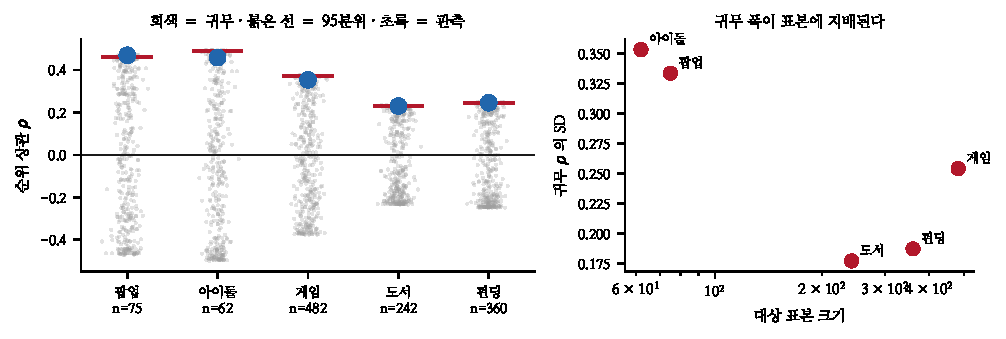
\includegraphics[width=\textwidth]{figs/nulldist.pdf}
\caption{대상별 귀무분포. 관측이 95분위에 붙어 있다.}
\end{figure}

\begin{table}[t]
\centering\tsize
\caption{귀무 $\rho$의 폭.}
\begin{tabular}{lrrrr}
\toprule
대상 & n & 귀무 SD & 95분위 & 관측 \\
\midrule
아이돌 & 62 & \textbf{0.353} & $+$0.490 & $+$0.458 \\
팝업 & 75 & 0.334 & $+$0.461 & $+$0.469 \\
도서 & 242 & \textbf{0.177} & $+$0.229 & $+$0.230 \\
펀딩 & 360 & 0.187 & $+$0.245 & $+$0.245 \\
게임 & 482 & 0.254 & $+$0.370 & $+$0.353 \\
\bottomrule
\end{tabular}
\end{table}

귀무 SD가 대상 도메인마다 두 배씩 차이 난다. 유의 여부가 전이 품질보다 대상
표본 크기에 더 크게 달려 있다는 뜻이다.

\claimx{유의 개수는 채택 판정에 쓸 수 없다. 귀무분포의 폭이 대상 도메인의 표본
크기에 지배되므로, 같은 품질의 전이라도 대상이 작으면 유의하지 않고 크면
유의하다. 판정은 평균 $\rho$로 한다.}{표본 크기를 통제한 검정을 만들었을 때
결론이 달라지면 이 처방이 성급한 것이다.}

\paragraph{귀무가 무엇인지 다시 보자}
이 귀무는 \emph{인자 공간은 그대로 두고 계수만 무작위로} 만든다. 인자 공간이
이미 대상 라벨과 정렬돼 있으면 무작위 방향도 꽤 맞는다. 그래서 관측이 95분위에
붙는 것은 검정이 가혹해서가 아니라 \textbf{인자 공간 자체가 일의 대부분을
하고 있다}는 사실을 드러낸다. 성분이 둘뿐이라 무작위 방향의 자유도가 작다.

\section{결정 넷을 재감사한다}

유의 개수로 채택한 결정이 넷 있었다.

\begin{figure}[t]
\centering

\includegraphics[width=\textwidth]{figs/audit.pdf}
\caption{과거 채택 결정을 평균 순위 상관으로 다시 잰 것.}
\end{figure}

\begin{table}[t]
\centering\tsize
\caption{재감사.}
\begin{tabular}{llrr}
\toprule
결정 & 판정 & 전 & 후 \\
\midrule
노트 37 공통 축 2$\to$3 & \textbf{유지} & 0.3301 & \textbf{0.3438} \\
노트 40 쌍별 정렬 & \textbf{유지} & 0.3724 & \textbf{0.3742} \\
노트 37 게임 매장축 켜기 & \textbf{철회} & 0.3438 & 0.3516$^\dagger$ \\
노트 39 이중 배선 & \textbf{철회} & 0.3439 & 0.3430 \\
\bottomrule
\end{tabular}
\end{table}

{\footnotesize $^\dagger$ 끄는 쪽 값이다. 켜면 0.3438이므로 노트 37의 결정을 되돌렸다.}

\paragraph{게임 매장 노출도}
노트 28이 껐고 노트 37이 켰다. 순위 기준으로 재니 끄는 쪽이 낫고, 이득이
\emph{게임을 대상으로 한 네 셀에 전부} 몰린다.

\begin{table}[t]
\centering\tsize
\caption{게임 매장 노출도 축을 끌 때의 $\rho$ 변화.}
\begin{tabular}{lrrr}
\toprule
셀 & 켬 & 끔 & 차이 \\
\midrule
아이돌 $\to$ 게임 & $+$0.302 & $+$0.374 & \textbf{$+$0.072} \\
펀딩 $\to$ 게임 & $+$0.309 & $+$0.353 & $+$0.044 \\
팝업 $\to$ 게임 & $+$0.309 & $+$0.343 & $+$0.034 \\
도서 $\to$ 게임 & $+$0.306 & $+$0.329 & $+$0.022 \\
\midrule
게임이 출처인 네 셀 & \multicolumn{3}{r}{평균 변화 $-$0.004} \\
\bottomrule
\end{tabular}
\end{table}

노트 28의 원래 판단이 옳았다. 다만 공통 축 목록에서 빼는 것은 아니다 --- 다른
세 도메인은 이 축을 관측하고, 쌍별 정렬이 도메인별 관측 차이를 허용하므로
게임만 두 축으로 정렬하면 된다.

\paragraph{쌍별 정렬의 진짜 가치}
재감사하다 알게 된 것이 있다. 전역 기준 정렬은 \emph{모든} 도메인이 같은 공통
축 집합을 관측해야 하므로 펀딩(둘만 관측)을 애초에 넣을 수 없다. 노트 40은
쌍별 정렬을 성적($+$0.0547$\to+$0.0561)으로 정당화했는데, 실제 가치는 성능이
아니라 \textbf{적용 가능성}이었다.

\section{상충은 지표 인공물이 아니었다}

노트 38과 40의 상충이 MAE 기준이었으니 새 자로 다시 재야 했다.

\begin{figure}[t]
\centering

\includegraphics[width=\textwidth]{figs/roles.pdf}
\caption{왼쪽 --- 도메인별 두 역할과 셀 간 폭. 오른쪽 --- 자기 상관과의 관계.}
\end{figure}

\begin{table}[t]
\centering\tsize
\caption{순위 기준 역할 분석.}
\begin{tabular}{lrrr}
\toprule
도메인 & 자기 $\rho$ & 대상으로 & 출처로 \\
\midrule
아이돌 & $+$0.471 & $+$0.480 & $+$0.311 \\
팝업 & $+$0.364 & $+$0.461 & $+$0.316 \\
게임 & $+$0.286 & $+$0.307 & $+$0.357 \\
펀딩 & $+$0.207 & $+$0.243 & $+$0.367 \\
도서 & $+$0.197 & $+$0.228 & $+$0.368 \\
\midrule
\multicolumn{2}{l}{자기 $\rho$와의 상관} & $+$0.959 & $-$0.952 \\
\bottomrule
\end{tabular}
\end{table}

MAE 기준의 $+$0.992와 $-$0.992보다 조금 약하지만 결론은 같다. \textbf{상충은
살아남았다.}

그리고 더 선명해진 것이 있다. 같은 대상이면 출처가 무엇이든 $\rho$가 거의 같다
--- 게임을 대상으로 한 네 셀이 0.329--0.374, 도서를 대상으로 한 넷이 0.223--0.230이다.
\textbf{대상 간 분산이 출처 간 분산의 18.1배다.}

\begin{quote}\fontsize{9.5}{11.5}\selectfont
노트 24가 ``대상이 출처보다 네 배 중요''를 얻었고 노트 33이 ``출처 선택은
무의미''로 밀고 갔다가 노트 38이 ``출처 배선은 유의미''로 정정했다. 순위 기준에서
보면 셋 다 맞다 --- 출처를 \emph{고르는} 것은 무의미하고(18.1배), 출처를
\emph{어떻게 재는지}는 유의미하다($-$0.952).
\end{quote}

\section{현재 상태}

\begin{table}[t]
\centering\tsize
\caption{되돌린 뒤. 다섯 도메인 · 쌍별 정렬 · 유도 $\lambda$.}
\begin{tabular}{lrr}
\toprule
& 평균 $\rho$ & 유의 \\
\midrule
노트 43 이전 & $+$0.3438 & 10/20 \\
\textbf{되돌린 뒤} & \textbf{$+$0.3516} & 7/20 \\
\bottomrule
\end{tabular}
\end{table}

유의가 10에서 7로 줄었지만 그것은 이제 판정 기준이 아니다.

\section{한계}

\begin{itemize}[leftmargin=1.1em,itemsep=0.15em]
\item 평균 $\rho$에 신뢰구간을 붙이지 않았다. 0.3438과 0.3516의 차이가 표본
      요동보다 큰지 확인하지 않았다.
\item 귀무분포를 ``인자 공간 고정, 계수 무작위''로 두었다. 인자 공간까지 무작위로
      만드는 더 강한 귀무를 쓰면 유의가 크게 늘 것이고, 어느 쪽이 옳은 질문인지
      정하지 않았다.
\item 표본 크기를 통제한 검정을 만들지 않고 판정 기준만 옮겼다.
\item 노트 38·39·40의 결론 중 MAE로 얻은 수치들을 전부 다시 재지는 않았다.
      상충 두 관계만 확인했다.
\item 노트 41 이전의 결정들(노트 34·35의 배선 변경 등)은 재감사하지 않았다.
      그때는 자기 상관을 기준으로 골랐고 그것은 눈금과 무관하지만, 확인은 필요하다.
\end{itemize}

\section{다음}

\begin{enumerate}[leftmargin=1.3em,itemsep=0.15em]
\item 평균 $\rho$의 붓스트랩 신뢰구간 --- 0.008 차이가 의미 있는지.
\item 노트 34·35의 배선 결정을 순위 기준으로 재감사한다.
\item 창작자 색인 완성 $\to$ 펀딩 매장 노출도 $\to$ 재검정.
\item 인자 공간이 일의 대부분을 한다면, 계수를 아예 쓰지 않는 전이(공통 축
      부호만 맞추기)와 비교해 볼 만하다.
\end{enumerate}

\vspace{0.6em}
\hrule height 0.3pt
\vspace{0.5em}
{\footnotesize
\textbf{참고문헌}\\[0.3em]
Spearman, C. (1904). The proof and measurement of association between two things.
\emph{American Journal of Psychology}, 15(1), 72--101.\\[0.15em]
Good, P. (2005). \emph{Permutation, Parametric, and Bootstrap Tests of
Hypotheses}, 3rd ed. Springer.\\[0.15em]
Ben-David, S. et al. (2010). A theory of learning from different domains.
\emph{Machine Learning}, 79(1--2), 151--175.\\[0.15em]
Schoppe, O. et al. (2016). Measuring the performance of neural models.
\emph{Frontiers in Computational Neuroscience}, 10, 10.\\[0.15em]
Schönemann, P. H. (1966). A generalized solution of the orthogonal Procrustes
problem. \emph{Psychometrika}, 31(1), 1--10.
}

\end{document}
